\documentclass[12pt,a4paper]{article}

\usepackage[utf8]{inputenc}
\usepackage[spanish]{babel}
\usepackage{palatino}
\usepackage{amsmath}
\usepackage{amssymb}
\usepackage{url}
\usepackage{hyperref}
\usepackage{enumerate}
\usepackage{geometry}
\usepackage{booktabs}
\usepackage{underscore}
\usepackage{longtable}
\usepackage{graphicx}
\usepackage{listings}
\usepackage{csquotes}
\usepackage{float}
\usepackage[backend=biber, sortcites=true, sorting=none]{biblatex}
\addbibresource{./TP2.biblatex}

\geometry{
  a4paper,
  left=2.5cm,
  right=2.5cm,
  top=3cm,
  bottom=3cm
}

\begin{document}

\title{Análisis de Datos para Ciberseguridad: Trabajo práctico 2}

\author{
  Alonso Araya Calvo \\
  Pedro Soto \\
  Sofia Oviedo \\
  Instituto Tecnológico de Costa Rica, \\
  Escuela de Ingeniería en Computación, \\
  Programa de Maestría en Ciberseguridad
}

\date{ 21 de setiembre de 2025 }
\maketitle

En este segundo trabajo practico se realizaron distintas tareas para implementar arboles de decisión, un modelo
de redes neuronales y una implementación de una arquitectura TabNet para clasificar todos los tipos de ataques encontrados en el dataset KDD99.

En este trabajo se enfocó en poder optimizar los modelos por medio de la herramienta Optuna y poder observar cómo los modelos evolucionan
respecto a los hiperparámetros que se modificaron, y la generación de todas las métricas de evaluación para demostrar
el rendimiento y poder compararlos con otras técnicas.

Los resultados obtenidos dieron paso a entender cómo funcionan las diferentes técnicas de clasificación y como se pueden optimizar los modelos para obtener mejores resultados,
así como las fortalezas de cada una con respecto a rendimiento, tiempo de entrenamiento, costo computacional y complejidad del código.

\section{Implementación de un árbol de decisión
  y random forests para clasificar todos los
tipos de ataques}

En esta sección se desarrolló la implementación de un árbol de decisión y
un random forest para clasificar todos los tipos de ataques encontrados en el dataset KDD99.

Para este efecto se utilizó la librería Scikit Learn que contiene la funcionalidad necesaria para
entrenar estos modelos sin tener que implementarlos desde cero. Asimismo, se utilizó la librería
Optuna que permite optimizar los hiperparámetros de los modelos fácilmente.

En las siguientes subsecciones se detallan los resultados obtenidos y los pasos realizados
para generar estos modelos.

\subsection{Generación de las particiones del dataset}

Para poder particionar el set de datos correctamente se desarrolló una función llamada
`split_dataset' que se encarga de partir el dataset en tres conjuntos: entrenamiento,
validación y prueba.

Para ello se utiliza la función `train_test_split' de Scikit Learn que permite particionar el dataset
en dos conjuntos: entrenamiento y prueba.
Después se utiliza la función `train_test_split' de Scikit Learn nuevamente para particionar el conjunto de entrenamiento
en dos conjuntos: entrenamiento y validación, por medio del cálculo del tamaño de la validación
respecto al conjunto restante.

También se utilizó la estratificación para poder garantizar que la distribución de las clases
en cada conjunto sea la misma que en el conjunto completo y la habilidad de poder
enviar por parámetro una semilla para reproducir los resultados.

Esta función `split_dataset' recibe ciertos parámetros que son:
\begin{itemize}
  \item df: DataFrame de pandas con los datos del dataset
  \item target_column: Nombre de la columna de las clases en string
  \item test_size: Proporción numérica del conjunto de prueba
  \item val_size: Proporción numérica del conjunto de validación
  \item random_state: Seed para poder reproducir los resultados si se desea
\end{itemize}

Y lo que finalmente retorna es una tupla con todas las particiones del dataset con la
forma (X_train, X_val, X_test, y_train, y_val, y_test).

Esta salida significa:

\begin{itemize}
  \item X_train: DataFrame con las características de entrenamiento
  \item X_val: DataFrame con las características de validación
  \item X_test: DataFrame con las características de prueba
  \item y_train: Series con las clases de entrenamiento
  \item y_val: Series con las clases de validación
  \item y_test: Series con las clases de prueba
\end{itemize}

El tamaño de cada conjunto se muestra en el Cuadro 1, mostrado a continuación:

\begin{table}[ht]
  \centering
  \begin{tabular}{lrr}
    \hline
    Conjunto        & Tamaño & Porcentaje \\
    \hline
    Completo        & 145586 & 100\% \\
    Entrenamiento   & 101910 & 70\% \\
    Validación      & 21838  & 15\% \\
    Prueba          & 21838  & 15\% \\
    \hline
  \end{tabular}
  \caption{Tamaño del conjunto y particiones de entrenamiento, validación y prueba.}
  \label{tab:particiones_kdd99}
\end{table}

Como se muestra en el Cuadro 1, el conjunto fue particionado correctamente, cumpliendo con el porcentaje esperado.

Para que las particiones fueran uniformes, se utilizó la estratificación para poder garantizar la distribución uniforme de las clases.

\begin{table}[h!]
  \centering
  \tiny
  \resizebox{\textwidth}{!}{
    \begin{tabular}{lrrrr}
      \hline
      Clase & Completo & Entrenamiento & Validación & Prueba \\
      \hline
      back.             & 0.006649 & 0.006653 & 0.006640 & 0.006640 \\
      buffer\_overflow. & 0.000206 & 0.000206 & 0.000183 & 0.000229 \\
      ftp\_write.       & 0.000055 & 0.000059 & 0.000046 & 0.000046 \\
      guess\_passwd.    & 0.000364 & 0.000363 & 0.000366 & 0.000366 \\
      imap.             & 0.000082 & 0.000079 & 0.000092 & 0.000092 \\
      ipsweep.          & 0.004472 & 0.004465 & 0.004488 & 0.004488 \\
      land.             & 0.000131 & 0.000128 & 0.000137 & 0.000137 \\
      loadmodule.       & 0.000062 & 0.000069 & 0.000046 & 0.000046 \\
      multihop.         & 0.000048 & 0.000049 & 0.000046 & 0.000046 \\
      neptune.          & 0.355941 & 0.355942 & 0.355939 & 0.355939 \\
      nmap.             & 0.001085 & 0.001079 & 0.001099 & 0.001099 \\
      normal.           & 0.603300 & 0.603297 & 0.603306 & 0.603306 \\
      perl.             & 0.000021 & 0.000020 & 0.000046 & 0.000000 \\
      phf.              & 0.000027 & 0.000029 & 0.000000 & 0.000046 \\
      pod.              & 0.001415 & 0.001413 & 0.001420 & 0.001420 \\
      portsweep.        & 0.002857 & 0.002865 & 0.002839 & 0.002839 \\
      rootkit.          & 0.000069 & 0.000069 & 0.000092 & 0.000046 \\
      satan.            & 0.006223 & 0.006221 & 0.006228 & 0.006228 \\
      smurf.            & 0.004403 & 0.004406 & 0.004396 & 0.004396 \\
      spy.              & 0.000014 & 0.000020 & 0.000000 & 0.000000 \\
      teardrop.         & 0.006306 & 0.006300 & 0.006319 & 0.006319 \\
      warezclient.      & 0.006134 & 0.006133 & 0.006136 & 0.006136 \\
      warezmaster.      & 0.000137 & 0.000137 & 0.000137 & 0.000137 \\
      \hline
    \end{tabular}
  }
  \caption{Distribución de clases en los conjuntos: completo, entrenamiento, validación y prueba.}
  \label{tab:dist_all}
\end{table}

Como es posible observar en el Cuadro 2, la distribución de clases de manera uniforme hace que se pueda
validar de una mejor manera los modelos, ya que se puede ayudar a que el modelo no se entrene
con una inclinación injustificada hacia cierto ataque y los splits sean más justos para evaluar el modelo en todas
sus clases.

\subsection{Entrenamiento, Optimización y Evaluación del Árbol de Decisión}

En esta sección se realizó la optimización de los parámetros del árbol de decisión con Optuna.
Se compararon los tres mejores arboles de decisión encontrados y se evaluaron mediante 10 corridas independientes,
generando particiones diferentes para cada corrida y calculando las métricas de evaluación. Finalmente se genero
una interpretación en base a los gráficos y tablas generados por los resultados de cada subsección.

\subsubsection{Optimización de Hiperparámetros con Optuna}

Como parte del trabajo se realizó la optimización de varios hiperparámetros para el árbol de decisión implementado con Scikit Learn.
Para este efecto se utilizó la librería Optuna en la cual se optimizaron los parámetros necesarios de la función `DecisionTreeClasifier' en
un estudio de 100 pruebas de optimización. Se entrenó con la partición de entrenamiento y se evaluó las predicciones con la partición de validación
utilizando como resultado el F1-Score promedio macro en base a la predicción con el conjunto de validación.

Para generar la optimización de los parámetros se creó la función `optimize_decision_tree' que se encarga de recibir por
parámetro un objeto de estudio de Optuna por medio de la función `create_study' y dentro de la función
de optimización se definen los rangos de los parámetros a optimizar,
se define la función del árbol de decisión de Scikit Learn y se entrena
con la partición de entrenamiento y se evalúa con la partición de validación
por medio de las funciones `predict', `fit' y
para generar la puntuación se utilizó `f1_score' de Scikit Learn que también
es utilizada como salida de la función de optimización.

Se optimizaron los siguientes hiperparámetros:

\begin{itemize}
  \item Profundidad máxima del árbol (max\_depth)
  \item Cantidad mínima de observaciones por partición (min\_samples\_split)
  \item Cantidad mínima de observaciones por hoja (min\_samples\_leaf)
  \item Criterio de pureza (criterion)
\end{itemize}

Para el parámetro de profundidad máxima del árbol se optimizo el valor en un rango de 3 a 20. Este rango se escogió debido
a las siguientes razones encontradas \autocite{sklearnerConfigureDecisionTreeClassifierMax_depth,scikitlearnDecisionTrees,christinaellisMaxDepthRandom2022}:
\begin{itemize}
  \item Valores muy bajos podrían causar que el árbol no capture los patrones del dataset correctamente y no genere un buen resultado,
    por lo que empezar con 3 es un buen valor inicial.
  \item Valores muy altos podrían permitir que el árbol se sobre ajuste y no generalice bien, por lo que 20 es un valor optimo.
  \item El valor límite de 20 es suficiente ya que más profundidad no se observa que mejoren el resultado y sería un desperdicio de cómputo.
  \item El dataset tiene clases desbalanceadas,
    por lo que profundidades muy altas podrían crear una inclinación hacia estas clases grandes.
\end{itemize}

En cuanto al parámetro de cantidad mínima de observaciones por partición se optimizo el valor en un rango de 2 a 50.
Las consideraciones fueron \autocite{mDecisionTreesSplit2024,gibbinsVisualGuideTuning2025}:
\begin{itemize}
  \item Los valores muy bajos como 2 podrían generar que el árbol se divida excesivamente y que se ajuste al ruido del dataset.
  \item Se deja el límite en 50 dado que valores bajos dan paso a más varianza y posibles sobre ajustes,
    mientras que los valores altos podrían permitir una mejor generalización, sin llegar al exceso
    que el árbol casi no se divida.
  \item El rango de 2 a 50 es lo suficientemente moderado para poder generar splits con buen soporte,
    pero tampoco tan pequeño como para que se generen splits débiles como serian con un valor bajo, evitando un árbol muy simple o especifico.
\end{itemize}

En el caso de la cantidad mínima de observaciones por hoja se optimizo el valor en un rango de 1 a 25.
Los puntos para tomar fueron \autocite{ConfigureDecisionTreeClassifierMin_samples_leaf,wijayaNBDLite42023}:
\begin{itemize}
  \item Valores bajos pueden crear hojas con muy pocos ejemplos, dando paso a que se
    sobre ajuste a cierto patrones específicos del dataset.
  \item Los valores altos podrían dar paso a poder generalizar mejor, ya que contiene un numero
    más alto de muestras, reduciendo la varianza y posiblemente evitando el sobre ajuste.
  \item Si se obtienen hojas con más datos es posible que los patrones aprendidos sean más estables.
  \item El valor límite de 25 permite suficientes hojas y reducir los nodos del árbol que podría
    mantener el árbol más pequeño y eficiente.
\end{itemize}

Por último, se optimizo el criterio de pureza en un rango de `gini' y `entropy'.
El criterio para este rango fue \autocite{raschkaWhyAreWe0000,aznarDecisionTreesGini2020}:
\begin{itemize}
  \item Se utiliza solo gini o entropy y no se incluye `log_loss' debido a que es más costoso computacionalmente y puede no dar una
    mejora significativa en contraste con los otros dos.
  \item Se incluye gini ya que es un algoritmo robusto y rápido computacionalmente.
  \item En el caso de entropy este es un poco más costoso que gini dado a que realiza el cálculo de logaritmos, pero puede
    llegar a ser un poco más preciso.
\end{itemize}

Para poder ejecutar esta función se creó un estudio de Optuna con la dirección de maximizar la función objetivo,
en este caso al escogerse como métrica el F1-Score promedio macro se buscó mejorar esta puntuación en todos los estudios.

Se realizaron 100 pruebas de Optuna, suficientes para poder encontrar las mejores tres arquitecturas en un tiempo adecuado,
su duración de ejecución en Google Colab fue de alrededor de un poco más de dos minutos,
mayores números de pruebas realmente no lo mejoraron significativamente por lo que no se justifica la computación
y tiempo mayor de estudio.

Se utilizo el F1-Score macro como la métrica a maximizar, debido a que el dataset KDD99 tiene clases desbalanceadas,
por lo que esta métrica permite dar importancia a todas las clases y no solo a algunas que son muy representativas
en este conjunto. Otras métricas como el accuracy podrían creer que es un buen modelo para cierto tipo de ataques
pero podría estar sesgado y otras clases podrían no ser detectadas correctamente con un rendimiento pobre.

\paragraph{Resultados y Demostración del Proceso de Optimización}

Para documentar el proceso de optimización se generaron distintos gráficos y tablas que permiten observar la evolución de cada estudio
realizado y la evolución de los parámetros, en especial de la métrica maximizada que fue el F1-Score, estos
gráficos fueron provistos por la librería Optuna por medio de su modulo optuna.visualization.

Los datos de los resultados finales se muestran en el Cuadro 3, 4 y 5, mostrado a continuación:

\begin{table}[htbp]
  \centering
  \begin{tabular}{l c}
    \hline
    Métrica & Valor \\
    \hline
    Número total de trials & 100 \\
    Mejor F1-macro & 0.8092 \\
    \hline
  \end{tabular}
  \caption{Resumen de la optimización con Optuna}
  \label{tab:optuna_resumen}
\end{table}

En el Cuadro 3 se observa como para 100 corridas de Optuna se obtuvo un mejor F1-Score de 0.8092,
siendo este un buen resultado al ser cercano al 1. Ejecuciones más largas mostraron resultados similares
por lo que se justifica el uso de 100 corridas para ahorrar cómputo y tiempo.

\begin{table}[htbp]
  \centering
  \begin{tabular}{l c}
    \hline
    Hiperparámetro & Valor \\
    \hline
    max\_depth & 17 \\
    min\_samples\_split & 7 \\
    min\_samples\_leaf & 1 \\
    criterion & gini \\
    \hline
  \end{tabular}
  \caption{Mejores hiperparámetros (según el mejor F1-macro)}
  \label{tab:optuna_mejores_hparams}
\end{table}

En el Cuadro 4 podemos determinar que los rangos utilizados para los parámetros tienen sentido,
dado que finalmente el max_depth se obtuvo un valor de 17, siendo este un valor alto pero no llegando al límite de 20.
El min_samples_split se obtuvo un valor de 7, siendo este un valor medio en el rango utilizado.
El min_samples_leaf se obtuvo un valor de 1 utilizando el mínimo valor del rango.
El criterion finalmente se utilizó gini como el mejor criterio, siendo este rápido y adecuado para la tarea.

\begin{table}[htbp]
  \centering
  \small
  \begin{tabular}{c c c c c c}
    \hline
    Arquitectura & F1-macro & max\_depth & min\_samples\_split & min\_samples\_leaf & criterion \\
    \hline
    1 & 0.8092 & 17 & 7  & 1 & gini \\
    2 & 0.7877 & 13 & 11 & 1 & gini \\
    3 & 0.7877 & 13 & 11 & 1 & gini \\
    \hline
  \end{tabular}
  \caption{Tres mejores arquitecturas encontradas}
  \label{tab:optuna_top3}
\end{table}

En el Cuadro 5 se muestran las tres mejores arquitecturas para el estudio realizado. Se observa que el criterio de
gini es el más determinante para este problema, así como el min_samples_leaf con su valor de 1. Además se observa que el
valor de max_depth y min_samples_split son similares pero tienden a variar un poco entre los modelos.

\begin{table}[H]
  \centering
  \begin{tabular}{l c}
    \hline
    Métrica & Valor \\
    \hline
    F1-score promedio & 0.6495 \\
    Desviación estándar & 0.0975 \\
    F1-score mínimo & 0.2717 \\
    F1-score máximo & 0.8092 \\
    \hline
  \end{tabular}
  \caption{Estadísticas de la optimización}
  \label{tab:optuna_stats}
\end{table}

En cuanto al Cuadro 6 se muestran las estadísticas de la optimización en cuando al F1-Score.
Donde se observa su promedio, desviación estándar, mínimo y máximo, siendo el máximo el mejor valor encontrado.

Para mostrar los resultados de la evolución de la optimización se generaron distintos gráficos mostrados en la Figuras 1, 2, 3 y 4,
que serían la historia de optimización del F1-Score, importancia de los hiperparámetros,
relaciones entre parámetros, distribuciones de los valores objetivo y una comparación de las tres mejores arquitecturas por F1-Score.

\begin{figure}[H]
  \centering
  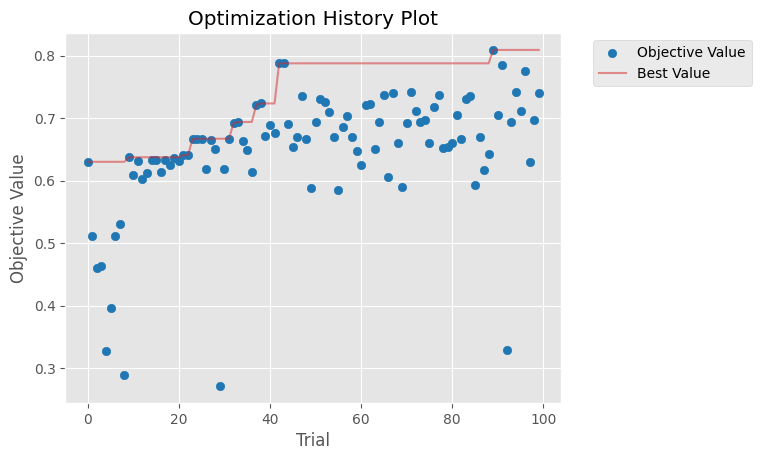
\includegraphics[width=0.8\textwidth]{../img/OptimizationHistory.png}
  \caption{Historia de optimización del F1-Score}\label{fig:decison-tree-optimization-history}
\end{figure}

En la Figura 1 se explica la evolución de la métrica objetivo que fue el F1-Score a lo largo de las 100 corridas.
Se puede apreciar la tendencia a la alza de la mejor puntuación pero también se observa las variaciones en la
métrica de forma muy dispersa a lo largo de las pruebas.
La mejor puntuación fue encontrada en la corrida 89, la cual fue la que genero el mejor F1-Score de 0.8092, las otras dos
mejores fueron encontradas alrededor de las pruebas entre 40 y 50.

\begin{figure}[H]
  \centering
  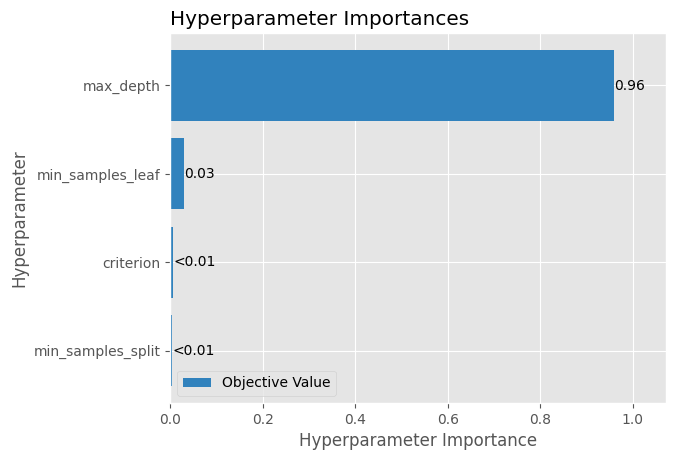
\includegraphics[width=0.8\textwidth]{../img/HyperparameterImportance.png}
  \caption{Importancia de los hiperparametros}\label{fig:decison-tree-hyperparameter-importance}
\end{figure}

En la Figura 2 se retrata cuáles fueron los hiperparámetros que tuvieron más incidencia para contribuir
con la mejora de la métrica objetivo. En este caso como podemos observar la profundidad máxima tiene una
importancia mucho más grande que las demás.
En este orden se dice que el parámetro más importante es el max_depth,
seguido por el min_samples_leaf, el min_samples_split y el criterion.

\begin{figure}[H]
  \centering
  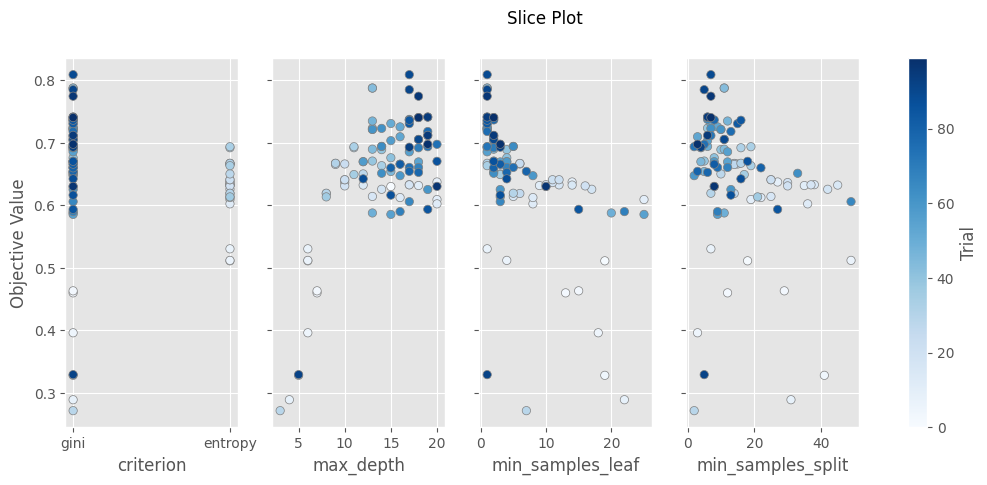
\includegraphics[width=0.8\textwidth]{../img/SliceDecisionTree.png}
  \caption{Relaciones entre hiperparámetros y la métrica objetivo}\label{fig:decison-tree-slice}
\end{figure}

En la Figura 3 se muestran como los hiperparámetros optimizados interactúan entre sí para generar el mejor F1-Score.
En esta grafica podemos ver la tendencia de cada uno de los parámetros
a cambiar su valor dentro del rango utilizado lo largo de las pruebas.
Se puede observar cómo alguna de estas tiende a quedarse en cierto grupo de valores,
en el caso de Gini, se ve como se utiliza más que el valor de Entropy, así como min_samples_leaf y min_samples_split
tienden a quedarse en valores del lado medio-bajo y finalmente el max_depth tiende a utilizar valores altos.

\begin{figure}[H]
  \centering
  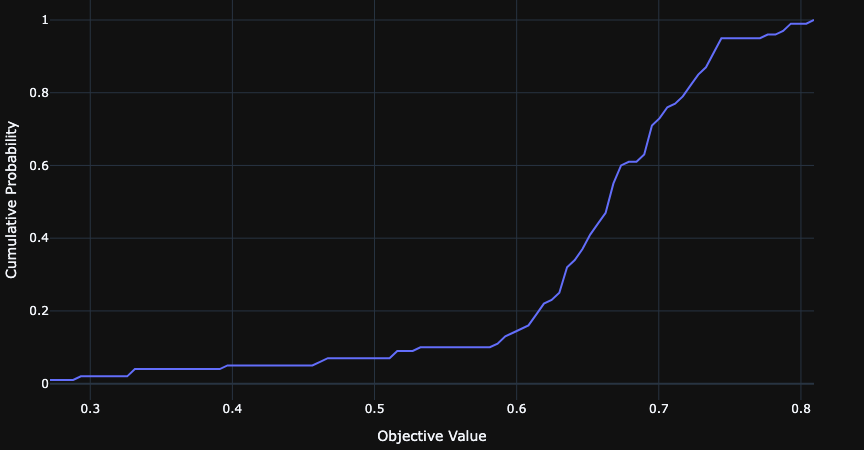
\includegraphics[width=0.8\textwidth]{../img/EDFDecisionTree.png}
  \caption{Distribución del valor objetivo}\label{fig:edf-decision-tree}
\end{figure}

La Figura 4 es una gráfica de distribución del valor objetivo que fue el F1-Score, se observa que
la puntuación estuvo en un rango entre alrededor de 0.3 y 0.8, siendo el 0.8 el mejor valor encontrado.
Además de eso se aprecia como la mayoría de las pruebas tuvieron una puntuación entre 0.6 y 0.8,
dando como resultado que con Optuna se encontraron buenos resultados en la mayoría de las pruebas.

\begin{figure}[H]
  \centering
  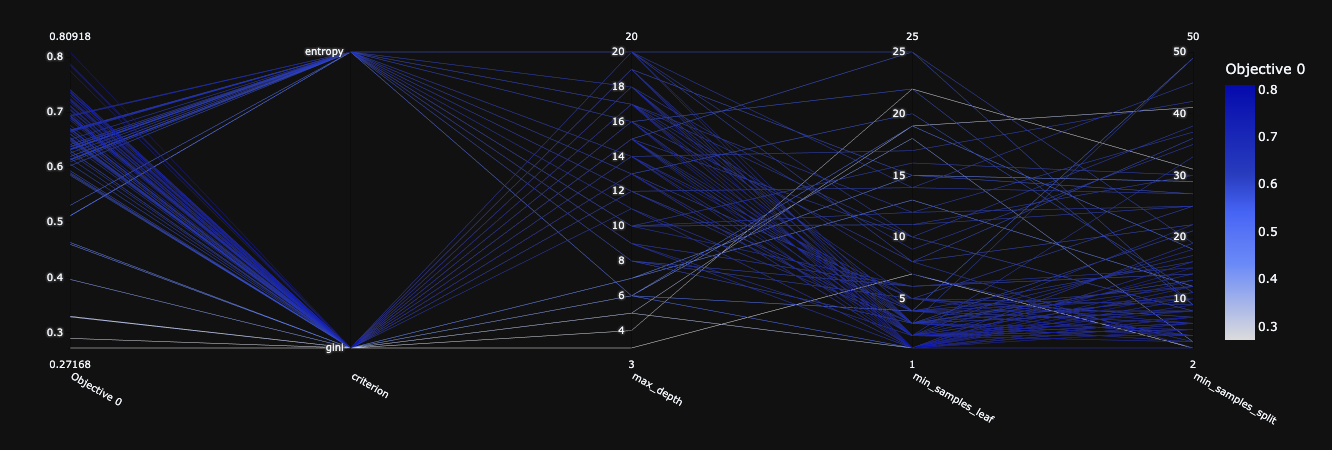
\includegraphics[width=1\textwidth]{../img/ParallelDecisionTree.png}
  \caption{Coordenadas paralelas: relación entre hiperparámetros y F1-macro}\label{fig:parallel-decision-tree}
\end{figure}

En la Figura 5 se observa que las mejores corridas por F1-macro (0.79 - 0.81)
se concentran en combinaciones con max_depth alto (13 - 17), min_samples_leaf de 1, min_samples_split (7 - 12)
y criterion de gini. Esto sugiere que el modelo se beneficia de árboles relativamente profundos con hojas pequeñas,
regulados por un umbral de división moderado. Al aumentar min_samples_leaf por encima de 1 o al reducir mucho la profundidad,
el desempeño tiende a degradarse. Asimismo, gini domina sobre entropy en este problema,
consistente con los tres mejores resultados encontrados del Cuadro 5.

\subsubsection{Comparación de las mejores arquitecturas con particiones diferentes}

En esta sección se comparan las tres mejores arquitecturas que se muestran en el Cuadro 5 y se evalúan
mediante 10 corridas independientes, generando particiones diferentes para cada corrida manteniendo la
proporción definida en la función `split_dataset' y calculando diferentes métricas
como el F1-Score, accuracy y tasa de falsos positivos para todas las evaluaciones.
Finalmente se recopilaron todos los resultados, y se calculó las medias
y desviaciones estándar de cada una de las arquitecturas y sus corridas.

Para poder lograr el objetivo de esta sección se guardaron los resultados de las tres mejores arquitecturas
en una lista para su uso posterior, este contenía los parámetros, posición y F1-Score de cada una de las arquitecturas.
Después se definió la función `evaluate_dt_architecture_multiple_runs' la cual va a estar encargada de:

\begin{itemize}
  \item Recibir los parámetros de la arquitectura a evaluar necesarias para la función `DecisionTreeClassifier' de Scikit Learn
    así como el número de corridas a realizar por arquitectura y semillas si es necesario para reproducibilidad.
  \item Se itera sobre el número de corridas y se generan las nuevas particiones por medio de la función `split_dataset'
  \item Se entrena el árbol de decisión con los parámetros recibidos y las nuevas particiones
  \item Se generan las predicciones por medio de la partición de prueba
  \item Se evalúa y se obtiene el F1-Score Macro, F1-Score por clase, accuracy y
    tasa de falsos positivos para todas las evaluaciones, siendo estos
    guardados en una lista individualmente
  \item Se retorna un diccionario con los resultados de las métricas calculadas como
    numero de corridas, parámetros, todos los F1-Score, accuracy, tasa de falsos positivos y matriz de confusión,
    además de las estadísticas como promedio y desviaciones de las métricas generadas.
\end{itemize}

Las métricas fueron calculadas mediante las funciones de Scikit Learn `f1_score', `accuracy_score', `precision_recall_fscore_support' y `confusion_matrix'.

Para el cálculo de la tasa de falsos positivos se utilizó la formula:

\begin{equation}
  FPR = \frac{FP}{FP + TN}
\end{equation}

Donde FP es el número de falsos positivos y TN es el número de verdaderos negativos.
Se utilizo la función `confusion_matrix' de Scikit Learn para obtener
la matriz de confusion y calcular los valores de FP y TN.

En los siguientes Cuadros 7, 8 y 9, se muestran las corridas realizadas y sus métricas.

\begin{table}[H]
  \centering
  \begin{tabular}{c c c c}
    \hline
    Corrida & F1 & Accuracy & FPR \\
    \hline
    1  & 0.7639 & 0.9988 & 0.0001 \\
    2  & 0.7294 & 0.9982 & 0.0001 \\
    3  & 0.7188 & 0.9982 & 0.0001 \\
    4  & 0.6905 & 0.9980 & 0.0002 \\
    5  & 0.7014 & 0.9981 & 0.0002 \\
    6  & 0.7413 & 0.9983 & 0.0001 \\
    7  & 0.7452 & 0.9982 & 0.0001 \\
    8  & 0.7432 & 0.9985 & 0.0001 \\
    9  & 0.8402 & 0.9984 & 0.0001 \\
    10 & 0.6797 & 0.9981 & 0.0002 \\
    \hline
  \end{tabular}
  \caption{Resultados – Arquitectura 1}
  \label{tab:corridas_arq1}
\end{table}

El Cuadro 7 exhibe como la Arquitectura 1 que era la que obtuvo la mejor puntuación, sigue mejorando un poco
más con estas particiones realizadas, inclusive llegando a obtener un F1-Score de 0.8402, siendo este un mejor resultado
al inicial con Optuna que se obtuvo de 0.8092.

\begin{table}[H]
  \centering
  \begin{tabular}{c c c c}
    \hline
    Corrida & F1 & Accuracy & FPR \\
    \hline
    1  & 0.7200 & 0.9979 & 0.0002 \\
    2  & 0.7110 & 0.9978 & 0.0002 \\
    3  & 0.6552 & 0.9972 & 0.0003 \\
    4  & 0.6768 & 0.9978 & 0.0002 \\
    5  & 0.6416 & 0.9981 & 0.0002 \\
    6  & 0.6390 & 0.9976 & 0.0002 \\
    7  & 0.6400 & 0.9978 & 0.0002 \\
    8  & 0.6782 & 0.9977 & 0.0002 \\
    9  & 0.6988 & 0.9976 & 0.0002 \\
    10 & 0.7262 & 0.9978 & 0.0002 \\
    \hline
  \end{tabular}
  \caption{Resultados – Arquitectura 2}
  \label{tab:corridas_arq2}
\end{table}

\begin{table}[H]
  \centering
  \begin{tabular}{c c c c}
    \hline
    Corrida & F1 & Accuracy & FPR \\
    \hline
    1  & 0.6737 & 0.9976 & 0.0002 \\
    2  & 0.6167 & 0.9974 & 0.0003 \\
    3  & 0.6483 & 0.9975 & 0.0002 \\
    4  & 0.7159 & 0.9974 & 0.0002 \\
    5  & 0.7049 & 0.9977 & 0.0002 \\
    6  & 0.6719 & 0.9973 & 0.0002 \\
    7  & 0.7013 & 0.9977 & 0.0002 \\
    8  & 0.6717 & 0.9972 & 0.0003 \\
    9  & 0.6704 & 0.9977 & 0.0002 \\
    10 & 0.6486 & 0.9970 & 0.0003 \\
    \hline
  \end{tabular}
  \caption{Resultados – Arquitectura 3}
  \label{tab:corridas_arq3}
\end{table}

En cuanto al Cuadro 8 y 9 al ser arquitecturas encontradas con configuración idéntica se tienen resultados similares,
en este caso a diferencia de la primera arquitectura no se mejoró su F1-Score inicial de 0.7877.

En general todas las particiones obtuvieron métricas buenas inclusive en casi todos los falsos positivos tienen valores
muy bajos y los F1-Score por clase también están cerca de 1, dando a entender que es posible que obtengan
pocas falsas detecciones y puedan clasificar en su mayoría correctamente las clases.

Para generar un resumen de todos los resultados y calcular las medias y desviaciones estándar de las métricas se generó una lógica
en el notebook la cual está encargada de utilizar todos los resultados guardados previamente de la función `evaluate_dt_architecture_multiple_runs'
que contiene una lista de los resultados de todas las evaluaciones, conteniendo los momentos estadísticos de
cada una de las métricas utilizadas para cada corrida por arquitectura, así como los parámetros utilizados para cada corrida.
Siguientemente la lógica genera una tabla y unos gráficos para visualización de la distribución y valores de las medias, además de la desviación estándar
para cada arquitectura y sus corridas para una mejor comparación.

\begin{table}[ht]
  \centering
  \tiny
  \begin{tabular}{lcccc}
    \hline
    Arquitectura & F1-macro Media & F1-macro Desviación Estándar & FPR Media & FPR Desviación Estándar \\
    \hline
    \#1 & 0.7353 & 0.0431 & 0.0001 & 0.0000 \\
    \#2 & 0.6787 & 0.0323 & 0.0002 & 0.0000 \\
    \#3 & 0.6723 & 0.0284 & 0.0002 & 0.0000 \\
    \hline
  \end{tabular}
  \caption{Resultados de las Corridas con Particiones Diferentes}
  \label{tab:corridas_part_dt}
\end{table}

\begin{figure}[H]
  \centering
  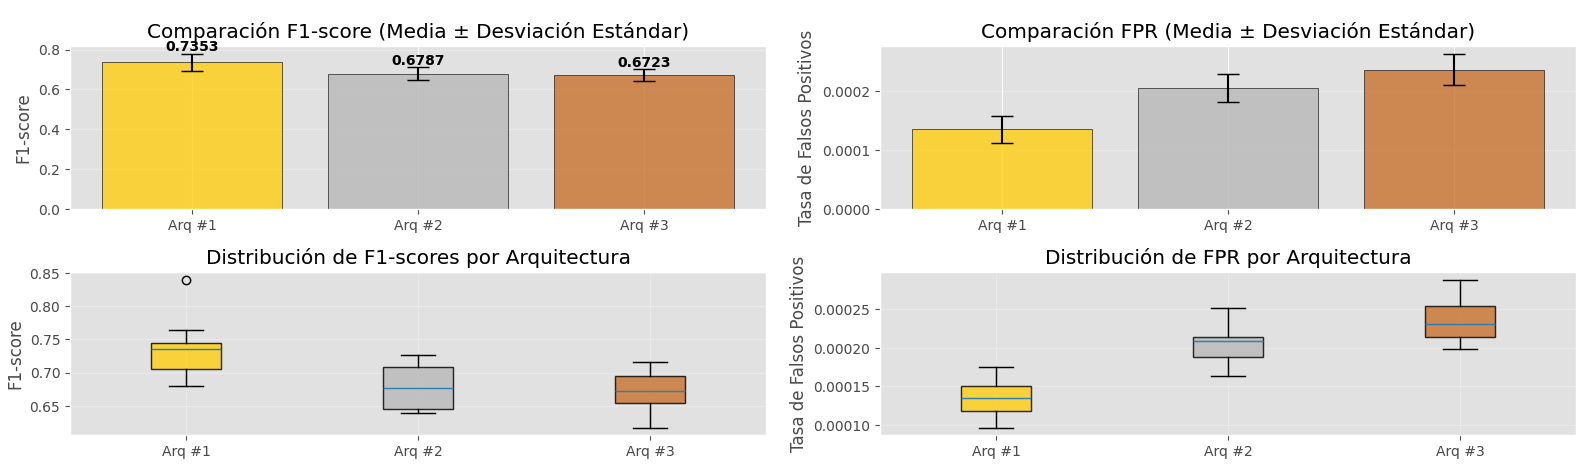
\includegraphics[width=1\textwidth]{../img/ComparacionPartArqui.png}
  \caption{Comparación de las Arquitectura con Particiones Diferentes}\label{fig:partition-architectures-decision-tree}
\end{figure}

En el Cuadro 10 y la Figura 6 se muestran los resultados generales por arquitectura para todas las 10 corridas realizadas para cada una.
En esta se reporta la media y desviación para las métricas que se utilizaron de F1-Score macro y tasa de falsos positivos.

En base al Cuadro 10 y la Figura 6 se pueden generar varias conclusiones de acuerdo con las arquitecturas encontradas:

\begin{itemize}
  \item La Arquitectura 1 es la que obtiene el mejor F1-Score macro y tasa de falsos positivos. Por ende
    sigue demostrando que es la mejor arquitectura en comparación a las arquitecturas 2 y 3.
  \item La Arquitectura 2 y 3 al tener los mismos parámetros son similares pero tienen una menor desviación en sus resultados
    dando a entender que son un poco más estables en sus resultados, la arquitectura 1 es más dispersa.
  \item Todas las arquitecturas presentan una tasa de falsos positivos muy baja, siendo este un buen resultado
    para el problema de detección de intrusos, ya que un aspecto importante es que se tengan pocas falsas detecciones
    y un sistema de este tipo sea más robusto.
\end{itemize}

\subsection{Entrenamiento, Optimización y Evaluación de un Random Forest}

En esta sección se realizó la optimización del parámetro `n_estimators' del Random Forest con Optuna,
este parámetro corresponde al número de árboles del Random Forest.
Se compararon los dos mejores Random Forests encontrados por Optuna y se evaluaron mediante 10 corridas independientes,
generando particiones diferentes para cada corrida y calculando las métricas correspondientes,
así como una interpretación final de todos los resultados generados.

\subsubsection{Optimización de Hiperparámetros con Optuna}

Similar a la sección 1.2 se realizó la optimización de los parámetros con Optuna, pero esta vez solamente
optimizando un RandomForest por medio de la función `RandomForestClassifier' de Scikit Learn.
Esto fue realizado en la función `optimize_random_forest' que se encarga de recibir por
parámetro un objeto de estudio de Optuna por medio de la función `create_study' y dentro de la función
de optimización se definió el único parámetro a optimizar que es el `n_estimators', este parámetro
indica la cantidad de árboles del Random Forest.
Además, se entrenó con la partición de entrenamiento y se evaluó con la partición de validación,
finalmente se utilizó el F1-Score macro como la métrica a maximizar y este era el valor que retornaba la función de optimización.

Se optimizo mediante la métrica de F1-Score macro, debido a las clases desbalanceadas del dataset KDD99, esto
permitía poder realizar un promedio sin considerar la frecuencia de las clases y poder dar una mejor
perspectiva del rendimiento general del modelo. Otras métricas podrían tener problemas en cuanto a sesgo de las clases
y pensar que es un buen modelo sin tomar en cuanta otras clases minoritarias y generando posiblemente un modelo
con muchas falsas alarmas

Se realizaron 50 pruebas de optimización debido al alto tiempo de ejecución y computo, en nuestros experimentos se observó que
la mayoría de las veces se obtenía el mejor resultado en corridas tempranas usualmente antes de la corrida 20, por lo que utilizar
más pruebas no se consideró necesario para efecto del trabajo, tomando como balance la computación y tiempo de corrida.
En nuestra ejecución en Google Colab el tiempo para ejecutar estos trials es de alrededor de siete minutos y medio.

Se optimizo el parámetro `n_estimators' en un rango de 10 a 300, este rango se escogió debido a que se observó que:
\begin{itemize}
  \item Si se utilizan pocos arboles el rendimiento es muy similar a utilizar un solo árbol,
    por lo que se puede considerar que 10 arboles es un buen valor inicial.
  \item En varios experimentos realizados la mejor solución se encontró en menos de 100 `n_estimators',
    por lo que se podría considerar que 300 es un valor suficiente para experimentar, esto también es apoyado por
    \autocite{probstHyperparametersTuningStrategies2019} donde menciona que en general hay
    rendimientos decrecientes después de 200 a 500 árboles.
  \item El costo computacional podría aumentar si se utilizan demasiados árboles y el rendimiento podría no mejorar
    en relación con el costo y tiempo computacional.
\end{itemize}

\paragraph{Resultados y Demostración del Proceso de Optimización}

Similar a los árboles de decisión se generaron gráficos y tablas para visualizar la evolución de la optimización.
Estos gráficos también fueron provistos por la librería Optuna por medio de su modulo optuna.visualization.

Como resultado del proceso de optimización se encontró el mejor parámetro n_estimator y F1-Score macro.
Esto se muestra en el siguiente Cuadro 11:

\begin{table}[htbp]
  \centering
  \begin{tabular}{lccc}
    \hline
    & Total de trials & Mejor F1-macro & \textit{n\_estimators} óptimo \\
    \hline
    Resultados & 50 & 0.7779 & 61 \\
    \hline
  \end{tabular}
  \caption{Resumen de la optimización de Random Forest con Optuna}
  \label{tab:optuna-rf-resumen}
\end{table}

Del Cuadro 11 se muestra un resultado optimo de 0.7779 en F1-Score macro, siendo este un buen resultado al ser más cercano al 1
y un numero de árboles moderado para el rango utilizado previamente que podía llegar hasta 300.

También, se calcularon las dos mejores arquitecturas que se muestran en el Cuadro 12:

\begin{table}[htbp]
  \centering
  \begin{tabular}{lcc}
    \hline
    Modelo & F1-macro & \textit{n\_estimators} \\
    \hline
    Random Forest \#1 & 0.7779 & 61 \\
    Random Forest \#2 & 0.7779 & 66 \\
    \hline
  \end{tabular}
  \caption{Top 2 modelos de Random Forest encontrados}
  \label{tab:optuna-rf-top2}
\end{table}

Del cuadro 12 observamos que las dos arquitecturas obtuvieron el mismo F1-Score macro y un numero de árboles muy similar.

En base a las siguientes figuras generadas sobre la evolución de la optimización se puede apreciar una mejor
perspectiva del proceso.

\begin{figure}[H]
  \centering
  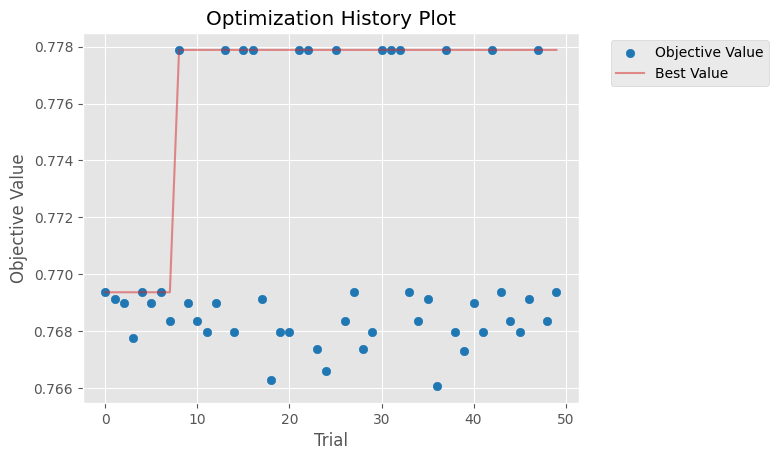
\includegraphics[width=0.8\textwidth]{../img/OptimizationHistoryDecisionForest.png}
  \caption{Histórico de Optimización del Random Forest}\label{fig:optimization-random-forest}
\end{figure}

En la Figura 7 se denota como mejoro el valor objetivo que fue nuestro F1-Score macro a lo largo de los estudios.
Se muestra como muy rápidamente desde menos de 10 trials se obtuvo el mejor resultado de las 50 pruebas,
también a lo largo de los trials se observan distintos puntos donde el F1-Score llego a un punto similar en
múltiples pruebas, lo que podría indicar que no es posible realmente mejorar por mucho el modelo
por más trials que se hagan para el rango de `n_estimators' utilizado. Además, se observa como en general
el Random Forest provee moderadamente buenos resultados, ya que la mayoría de las pruebas obtuvieron un F1-Score macro
entre 0.76 y 0.77.

\begin{figure}[H]
  \centering
  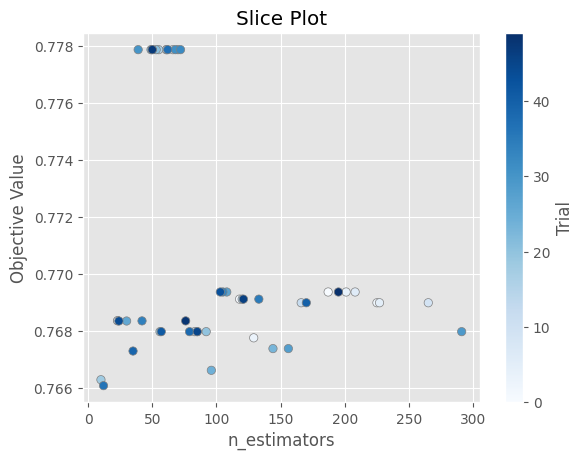
\includegraphics[width=0.8\textwidth]{../img/SlicePlotRandomForest.png}
  \caption{Relación entre hiperparámetros y F1-macro}\label{fig:slice-plot-random-forest}
\end{figure}

En esta Figura 8 se encuentra con el mejor optimo entre alrededor de 40 a 80 árboles, indicando que para el numero
de pruebas realizadas no es necesario utilizar muchos más árboles para obtener un mejor rendimiento, ya que
los rangos mayores al 80 se estancan en valores similares o menores, lo que no justificarían un numero alto
de árboles debido al costo computacional y tiempo de entrenamiento, inclusive al utilizar
un numero de árboles altos como se ve en algunas de estas pruebas de 200+ no se observa una mejoría significativa.

\begin{figure}[H]
  \centering
  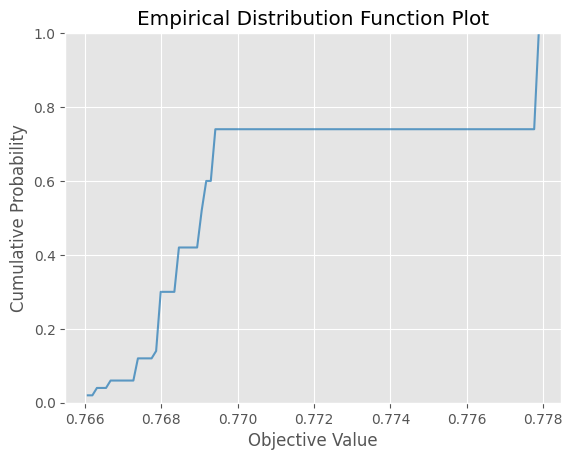
\includegraphics[width=0.8\textwidth]{../img/EDFRandomForest.png}
  \caption{Distribución del Valor Objetivo}\label{fig:edf-random-forest}
\end{figure}

De la Figura 9 se muestra que un aproximado del 75\% de las configuraciones de `n_estimators'
obtuvieron un F1-Score macro entre 0.76 y 0.77, y solo una prueba obtuvo un F1-Score macro de 0.779, en general
las puntuaciones fueron bastante similares y hasta existe un punto plano en el que el valor se mantiene constante
hasta llegar al valor máximo.

\begin{table}[H]
  \centering
  \begin{tabular}{lc}
    \hline
    Métrica & Valor \\
    \hline
    F1-score promedio & 0.7708 \\
    Desviación estándar & 0.0042 \\
    F1-score mínimo & 0.7661 \\
    F1-score máximo & 0.7779 \\
    \hline
  \end{tabular}
  \caption{Estadísticas de la optimización de Random Forest}
  \label{tab:rf-opt-stats}
\end{table}

Finalmente en el Cuadro 13 podemos ver los momentos estadísticos de la optimización de Random Forest,
donde se observa el promedio del F1-Score siendo un valor moderadamente alto debido a que fueron muy similar en las corridas,
una desviación estándar moderada debido a que no existe mucha dispersión en las puntuaciones y esto es soportado
por los máximos y mínimos donde se ve que no fueron valores muy distantes.

\subsubsection{Comparación de los dos mejores Random Forests con particiones diferentes}

Similar a la implementación de árboles de decisión, en esta parte se compararon solamente dos arquitecturas de
Random Forest que fueron encontradas después de 50 pruebas optimizando la cantidad de árboles con Optuna, estas se
puede observar en el Cuadro 12.

Para efectos de esta tarea se generó una función llamada `evaluate_rf_architecture_multiple_runs' que se encarga de recibir
los parámetros guardados anteriormente de los RandomForests encontrados, el número de corridas a realizar y una lista de seeds aleatorias
para reproducir los experimentos.

Esta función itera sobre el número de corridas, se generan nuevas particiones mediante la función `split_dataset' realizada en la
primera parte y se extrae los conjuntos de entrenamiento y prueba, se entrena el Random Forest con los parámetros recibidos
y se generan las predicciones con el conjunto de prueba, se calculan las métricas de F1-Score macro, F1-Score por clase, accuracy, tasa de
falsos positivos, precision y recall por clase, además de la matriz de confusion, todos los resultados fueron recopilados,
se generaron momentos estadísticos para las métricas y fueron guardados en una variable para uso posterior en las siguientes celdas.

Esta función se ejecutó para las dos arquitecturas y se encontraron los siguientes resultados en el Cuadro 14 y 15:

\begin{table}[H]
  \centering
  \begin{tabular}{rccc}
    \hline
    Corrida & F1-macro & Accuracy & FPR \\
    \hline
    1  & 0.8266 & 0.9991 & 0.0001 \\
    2  & 0.8361 & 0.9994 & 0.0001 \\
    3  & 0.7790 & 0.9995 & 0.0000 \\
    4  & 0.7570 & 0.9991 & 0.0001 \\
    5  & 0.7698 & 0.9994 & 0.0001 \\
    6  & 0.8057 & 0.9991 & 0.0001 \\
    7  & 0.7323 & 0.9989 & 0.0001 \\
    8  & 0.7655 & 0.9990 & 0.0001 \\
    9  & 0.8443 & 0.9993 & 0.0001 \\
    10 & 0.8820 & 0.9994 & 0.0001 \\
    \hline
  \end{tabular}
  \caption{Resultados por corrida del Random Forest \#1 (n\_estimators = 61)}
  \label{tab:rf1-corridas}
\end{table}

\begin{table}[H]
  \centering
  \begin{tabular}{rccc}
    \hline
    Corrida & F1-macro & Accuracy & FPR \\
    \hline
    1  & 0.8865 & 0.9995 & 0.0000 \\
    2  & 0.6743 & 0.9992 & 0.0001 \\
    3  & 0.6932 & 0.9991 & 0.0001 \\
    4  & 0.8408 & 0.9992 & 0.0001 \\
    5  & 0.8618 & 0.9990 & 0.0001 \\
    6  & 0.8302 & 0.9994 & 0.0001 \\
    7  & 0.8782 & 0.9995 & 0.0000 \\
    8  & 0.7747 & 0.9991 & 0.0001 \\
    9  & 0.6997 & 0.9990 & 0.0001 \\
    10 & 0.7704 & 0.9992 & 0.0001 \\
    \hline
  \end{tabular}
  \caption{Resultados por corrida del Random Forest \#2 (n\_estimators = 66)}
  \label{tab:rf2-corridas}
\end{table}

Como se observa en los Cuadros 14 y 15 se obtuvieron resultados muy similares para las dos arquitecturas.
En este caso se observa que el F1-Macro aumento considerablemente respecto al mejor F1-Score macro
obtenido en el proceso de optimización, como se puede leer, el mejor F1-Score macro fue de 0.7779 y ahora
con estas particiones diferentes se obtuvieron valores entre 0.82 y 0.88, esto es un aumento considerable respecto
a lo inicial. Además de esto, en ambas arquitecturas se observan valores de accuracy de 0.99+ indicando una buena
capacidad de clasificar correctamente las clases y una tasa de falsos positivos muy baja, indicando que
el modelo podría no tener muchas falsas alarmas, perfecto para un sistema de detección de intrusos.

En el caso de esta comparación podemos ver que el mejor F1-Score macro fue el de la Arquitectura 2,
con un F1-Score macro de 0.8865 y una tasa de falsos positivos de 0. Sin embargo, podemos ver que la Arquitectura 1
es más estable ya que el rango de su F1-Score es menos variable entre corridas, el de la Arquitectura 2 es más variable
y sus valores por ende son más dispersos, por lo que la Arquitectura 1 es más consistente y confiable.

Otro punto para recalcar es que ambos usaron una cantidad de estimadores similares de 61 y 66, y tienen
una variabilidad moderada en sus resultados por lo que indica que este parámetro tiene un nivel de impacto a considerar.

\begin{table}[htbp]
  \centering
  \small
  \begin{tabular}{cccccccc}
    \hline
    Random & n\_estimators & F1-macro & F1-macro & Accuracy & Accuracy & FPR & FPR \\
    Forest &  & Media & Desv Std & Media & Desv Std & Media & Desv Std \\
    \hline
    \#1 & 61 & 0.7998 & 0.0444 & 0.9992 & 0.0002 & 0.0001 & 0.0000 \\
    \#2 & 66 & 0.7910 & 0.0761 & 0.9992 & 0.0002 & 0.0001 & 0.0000 \\
    \hline
  \end{tabular}
  \caption{Resumen de evaluación de los mejores Random Forests}
  \label{tab:rf-resumen-evaluacion}
\end{table}

\begin{figure}[H]
  \centering
  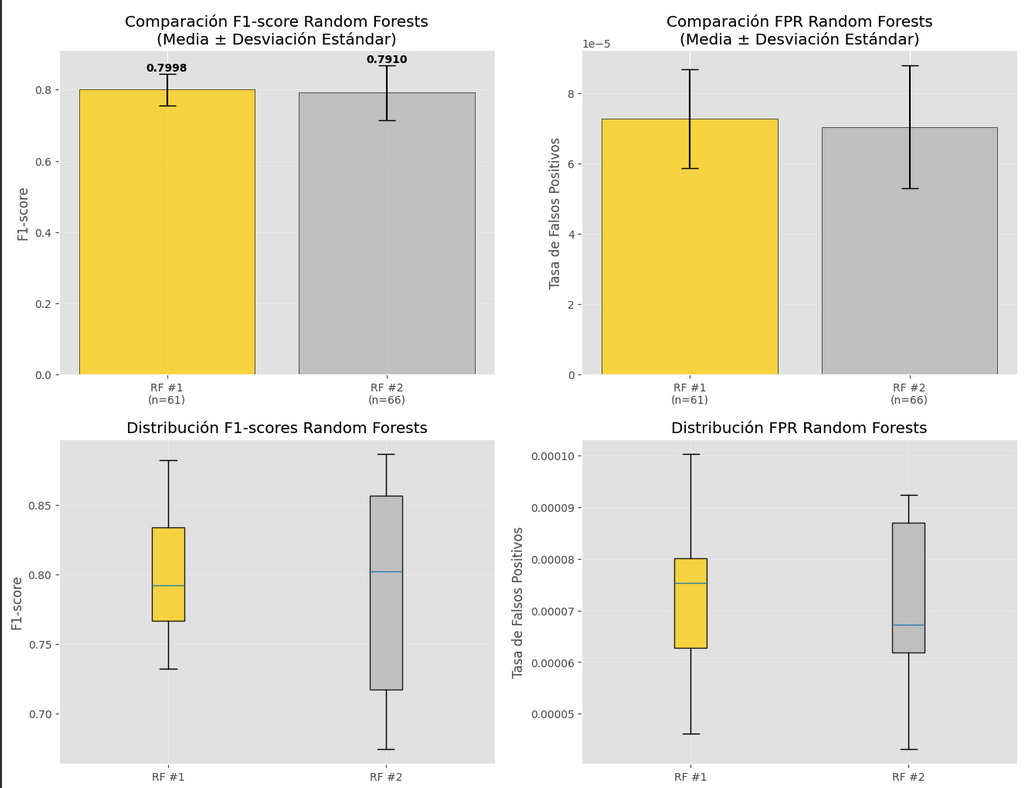
\includegraphics[width=0.8\textwidth]{../img/ComparacionRandomForest.png}
  \caption{Comparación de los dos mejores Random Forests}\label{fig:comparison-random-forest}
\end{figure}

En el Cuadro 16 y la Figura 10 podemos ver una comparación de las estadísticas de los resultados de la corrida
de las particiones por cada arquitectura, esto recalca los comentarios anteriores de que la Arquitectura 1 tiene menor
dispersión y es más estable, la tasa de falsos positivos es baja en ambos y casi que iguales por lo que
son buenos modelos iniciales para un sistema de detección de intrusos.

En general se podría decir que ambos son similares pero la Arquitectura 1 presenta menos dispersión en los resultados
y usa menos árboles para su modelo por lo que es más eficiente y tiene un buen rendimiento. Esto a nivel general
también nos dice que los Random Forests presentan buenos resultados con pocas modificaciones respecto a sus parámetros,
ya que en este caso solo se modificaron los `n_estimators' y se dejaron los valores defecto de scikit learn.
Existe la posibilidad de que se pueda mejorar más el rendimiento de ambos modelos con otros parámetros optimizados.

{\tiny
  \printbibliography[title={Referencias}]
}

\end{document}
